\section{Correctness of our algorithm} \label{sec:correct}

We prove that the matching $M$ output by Algorithm~\ref{algo:criRSM} is 
\begin{enumerate} [(I)]
    \item  Critical as well as relaxed stable (\RWSM) and
    \item  A $\frac{3}{2}$ approximation to the maximum size $\CRWSM$ in $G$.
\end{enumerate}
The proofs of claims marked with $\star$ are deferred to Appendix.

%Our correctness proof involves showing that the matching $M$ is -- (i) critical, (ii) relaxed stable and  (iii) $\frac{3}{2}$-approximation to the maximum size $\CRWSM$ in an instance $G$ of the \SMTTLQ\ problem
The partition of vertices defined below based on the levels of vertices in $\AA$ and the matching $M$ is useful for us. 
%In order to prove the correctness, we partition the vertices of $\AA\cup\BB$ into subsets and establish some properties about these sets. 

%\vspace{0.1in}


\noindent \textbf{Partition of vertices:} 
%We partition the vertex set $\AA\cup\BB$ as described next. 
The vertex set $\AA$ is partitioned into $\AA_0\cup\AA_1\cup\ldots\cup\AA_{\T}\cup\ldots\cup\AA_{\S+\T}$, and the vertex set $\BB$ is partitioned into $\BB_0\cup\BB_1\cup\ldots\cup\BB_{\T}\cup\ldots\cup\BB_{\S+\T}$. For every matched vertex $a\in\AA$ there exists $x\in\{0,\ldots,\S+\T\}$ such that $(a^x,b)\in M$. We use $x$ to partition the vertex set. Note that if  $(a^{\T^*},b)\in M$ then for the purpose of partitioning we consider $\T^*=\T$  as $\T^*$ is a sub-level of the level $\T$.
\begin{itemize}
    \item \label{itm:part111} \textbf{Matched vertices in $\AA\cup \BB$:} Let $a\in \AA, b\in \BB$ and $(a^x,b)\in M$ for some $x\in\{0,\ldots,\S+\T\}$. Then we add $a$ to $\AA_x$ and $b$ to $\BB_x$.

    \item \label{itm:part411}{\bf Unmatched vertices in $\AA\cup\BB$:} 
    \begin{itemize}
        \item If a non-critical vertex $a\in \AA$ is unmatched in $M$ then we add $a$ to $\AA_{\T}$.
        \item If a critical vertex $a\in \AA$ is unmatched in $M$ then we add $a$ to $\AA_{\S+\T}$.
    % \end{itemize}



    
    % \item \label{itm:part5}\textbf{Unmatched vertices in $\BB$:}
    % \begin{itemize}
        \item If a non-critical vertex $b\in \BB$ is unmatched in $M$ then we add $b$ to $\BB_{\T}$.
        \item If a critical vertex $b\in \BB$ is unmatched in $M$ then we add $b$ to $\BB_0$.
        %=====================================================================================================
%=====================================================================================================

\begin{procedure}%
    \caption{TiesPropose($a^\ell,\prefal, M, Q$)}\label{proce:TiesProp} %( Kir{\'a}ly's algorithm~\cite{Kiraly13})
    \DontPrintSemicolon
    \SetAlgoLined
                Let $b$ be the favourite neighbour of $a$ in $\prefa$ at rank $k$\label{alg:favNbr}\; 
            \textbf{if} $b$ was marked by $a$ \textbf{then} $a$ unmarks $b$\;
            \If{$b$ is unmatched}{
                $M=M\cup \{(a^\ell,b)\}$\;
                \If{there exists an unmatched $b''$ at rank $k$ in $\prefa$ }{
                    Set $(a^\ell,b)$ as uncertain proposal}
            }
            \uElseIf{$b$ is part of an uncertain proposal $(a_j^y,b)$}{
                $M=(M\setminus \{(a_j^y,b)\}) \cup \{(a^\ell,b)\}$\;
                $a_j^y$ marks $b$ and add $a_j^y$ to $Q$}
            \uElseIf{$b$ is not part of an uncertain proposal}{
                Let $a_j^y= M(b)$\;
                \If{$\ell==\T$}{                   
                    \If{($y<\T$) or (($y==\T$ or $y==\T^*$) and $a\succ_b a_j$)}{
                        $M=M\setminus \{(a_j^y,b)\}\cup \{(a^\ell,b)\}$ and add $a_j^y$ to $Q$\;}
                    \textbf{else } add $a^\ell$ to $Q$
                }
                \If{$\ell==\T^*$}{                   
                    \If{($y<\T$) or ($y==\T$ and $a\succeq_b a_j$) or ($y==\T^*$ and $a\succ_b a_j$)}{
                    $M=M\setminus \{(a_j^y,b)\}\cup \{(a^\ell,b)\}$ and add $a_j^y$ to $Q$\;}
                    \textbf{else } add $a^\ell$ to $Q$
                }                
                }
\end{procedure}
\setlength{\intextsep}{8pt}% Remove \textfloatsep

%===============================================================================================================
%===============================================================================================================

    \end{itemize}
\end{itemize}



It is convenient to visualize the partitions as shown in Figure~\ref{fig:maxlevelgraph11}. This particular drawing of the graph $G$ is denoted by $G_M$ throughout the rest of the section. It is useful to assume that the edges in $G_M$ are implicitly directed from $\AA$ to $\BB$. By construction, the edges of $M$ (shown in blue colour) are horizontal whereas the unmatched edges (shown as solid black edges) can be horizontal, upwards or downwards.  

We state the properties of the vertices and edges in $G_M$ with respect to this partition in Property~\ref{property:GM}. % which is justified in the appendix.  
We briefly justify the properties in Property~\ref{property:GM} as follows. Only critical vertices in $\AA$ attain levels above $\T$. This implies that the partition set $\AA_{\T+1},\ldots,\AA_{\S+\T}$ contain only critical $a\in\AA$. Thus, we have Property~\ref{property:GM}(\ref{obs:partitionPorp2}).
Since each $a\in\AA$ at a level at most $\T-1$ does not propose to any non-critical vertex, the matched partner of each $a^x$ for $x\le \T-1$ is a critical vertex. Also, all the unmatched non-critical vertices on $\BB$-side are only in $\BB_{\T}$. This implies that the partition set $\BB_0,\ldots,\BB_{\T-1}$ contain only critical $b\in\BB$.  Thus, we have Property~\ref{property:GM}(\ref{obs:partitionPorp1}). 
 If a vertex $a$ remains unmatched in $M$ then by the design of our algorithm it must have exhausted its preference list at level $\S+\T$ (if it is a critical vertex) or at level $\T$, more specifically $\T^*$, (if it is a non-critical vertex)  and got rejected by each of its neighbours. Recall that each $b$ prefers a higher level $a$ over any lower level $a'$ irrespective of the ranks of $a$ and $a'$ in $\prefb$. Thus, Property~\ref{property:GM}(\ref{obs:partitionPorp4}) and Property~\ref{property:GM}(\ref{obs:partitionPorp3}) hold in $G_M$. Observe that if any vertex $b\in\BB$ receives a proposal then it cannot remain unmatched in $M$. This implies, if a critical $b$ is unmatched then none of its neighbours has proposed it at level 0, which further implies that they have not exhausted $\prefslqa$ at level 0. By construction, $b$ is in $\BB_0$. Hence, we have Property~\ref{property:GM}(\ref{obs:partitionPorp5}). Similarly, if $b$ is non-critical and unmatched then none of its neighbours can go to level $\T+1$ or above. By construction, $b$ is in $\BB_{\T}$. Hence, we have Property~\ref{property:GM}(\ref{obs:partitionPorp6}).

% Since each $a\in\AA$ at a level at most $\T-1$ proposes to vertices in $\prefslqa$ and only deficient $a$ raises its level above $\T$. The above partition and the matching $M$ implies that the partition set $\BB_0,\ldots,\BB_{\T-1}$ contain only critical $b\in\BB$ and all non-critical $b\in\BB$ are in $\BB_{x}$ for $x\ge \T$. Similarly, the partition set $\AA_{\T+1},\ldots,\AA_{\S+\T}$ contain only critical $a\in\AA$ and all non-critical $a\in\AA$ are in $\AA_{x}$ for $x\le \T$. Thus, we have Property~\ref{property:GM}(\ref{obs:partitionPorp1}) and Property~\ref{property:GM}(\ref{obs:partitionPorp2}). If a vertex $a$ remains unmatched in $M$ then by the design of our algorithm it must have exhausted its preference list at level $\T$, more specifically $\T^*$, (if it is a non-critical node) or at level $\S+\T$ (if it is a critical node) and got rejected by each of its neighbours. Recall that each $b$ prefers a higher level $a$ over any lower level $a'$ irrespective of the ranks of $a$ and $a'$ in $\prefb$. Thus, Property~\ref{property:GM}(\ref{obs:partitionPorp3}) and Property~\ref{property:GM}(\ref{obs:partitionPorp4}) hold in $G_M$. Observe that if any vertex $b\in\BB$ receives a proposal then it cannot remain unmatched in $M$. This implies that an unmatched $b$ did not receive any proposal. Thus, we have Property~\ref{property:GM}(\ref{obs:partitionPorp5}) and Property~\ref{property:GM}(\ref{obs:partitionPorp6}).


\begin{figure}
\begin{center}
    \scalebox{0.8}{
	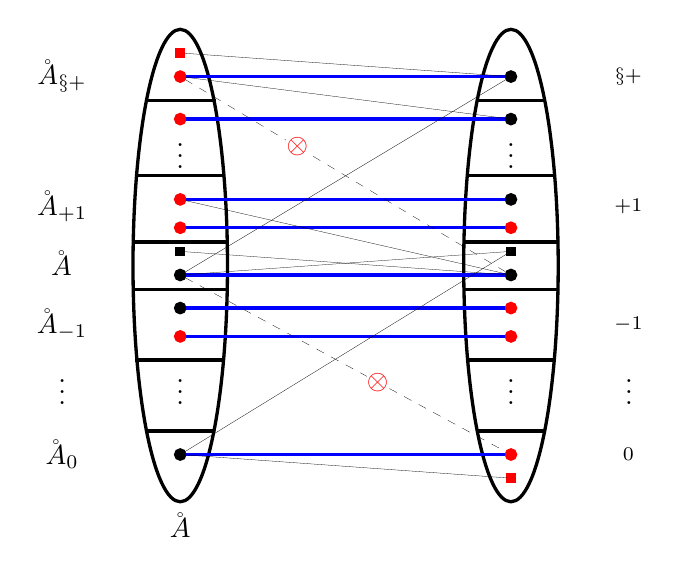
\begin{tikzpicture}[scale=0.6, thick,fsnode/.style={draw,circle,fill=black,scale=0.4}, lnode/.style={draw=red,circle,fill=red,scale=0.4}, snode/.style={draw=blue,circle,fill=blue,scale=0.4},tnode/.style={draw=black,fill=black,scale=0.4}, ltnode/.style={draw=red,fill=red,scale=0.4}]
	% ----------------A0'--------------------%
	\draw[very thick] (1,1.5) ellipse (1cm and 5cm);
	\node at (1,-4) {$\AA$};
	\draw[very thick] (0.25,5) -- (1.75,5);
	\node at (1,4) {\vdots};
	\draw[very thick] (0.07,3.4) -- (1.93,3.4);
	\draw[very thick] (0,2) -- (2,2);
	\draw[very thick] (0,1) -- (2,1);
	\node at (1,-1) {\vdots};
	\draw[very thick] (0.05,-0.5) -- (1.95,-0.5);
	\draw[very thick] (0.3,-2) -- (1.7,-2);
	\node at (-1.5,5.5) {$\AA_{\S+\T}$};
	\node at (-1.5,2.75) {$\AA_{\T+1}$};
	\node at (-1.5,1.5) {$\AA_{\T}$};
	\node at (-1.5,0.25) {$\AA_{\T-1}$};
	\node at (-1.5,-1) {\vdots};
	\node at (-1.5,-2.5) {$\AA_{0}$};
% 	% -------------B0'--------------%
	\draw[very thick] (8,1.5) ellipse (1cm and 5cm);
	\node at (8,-4) {$\BB$};
	\draw[very thick] (7.25,5) -- (8.75,5);
	\node at (8,4) {\vdots};
	\draw[very thick] (7.07,3.4) -- (8.93,3.4);
	\draw[very thick] (7,2) -- (9,2);
	\draw[very thick] (7,1) -- (9,1);
	\node at (8,-1) {\vdots};
	\draw[very thick] (7.05,-0.5) -- (8.95,-0.5);
	\draw[very thick] (7.3,-2) -- (8.7,-2);
	\node at (10.5,5.5) {$\BB_{\S+\T}$};
	\node at (10.5,2.75) {$\BB_{\T+1}$};
	\node at (10.5,1.5) {$\BB_{\T}$};
	\node at (10.5,0.25) {$\BB_{\T-1}$};
	\node at (10.5,-1) {\vdots};
	\node at (10.5,-2.5) {$\BB_0$};
% 	% ----------matched edges--------------%  
	\node[fsnode] (b3) at (8,5.5) {};
	\node[lnode] (a4) at (1,5.5) {};
	\draw[very thick,blue] (a4) -- (b3);
	\node[lnode] (a5) at (1,4.6) {};
	\node[fsnode] (b4) at (8,4.6) {};
    \draw[very thick,blue] (a5) -- (b4);
    \node[fsnode] (a2) at (1,0.6) {};
	\node[lnode] (b2) at (8,0.6) {};
	\draw[very thick,blue] (a2) -- (b2);
    \node[lnode] (a10) at (1,0) {};
	\node[lnode] (b10) at (8,0) {};
	\draw[very thick,blue] (a10) -- (b10);
    \node[lnode] (a9) at (1,2.9) {};
	\node[fsnode] (b9) at (8,2.9) {};
    \draw[very thick,blue] (a9) -- (b9);
    \node[lnode] (a11) at (1,2.3) {};
	\node[lnode] (b11) at (8,2.3) {};
    \draw[very thick,blue] (a11) -- (b11);
	\node[fsnode] (a6) at (1,1.3) {};
	\node[fsnode] (b5) at (8,1.3) {};
	\draw[very thick,blue] (a6) -- (b5);
	\node[fsnode] (a8) at (1,-2.5) {};
	\node[lnode] (b8) at (8,-2.5) {};
	\draw[very thick,blue] (a8) -- (b8);
	\node[ltnode] (b6) at (8,-3) {};
	\node[ltnode] (a1) at (1,6) {};
	\node[tnode] (b7) at (8,1.8) {};
	\node[tnode] (a7) at (1,1.8) {};
% 	%------------other edges---------------%  
	\draw[ultra thin] (a4) -- (b4);
	\draw[ultra thin] (a6) -- (b3);
	\draw[ultra thin] (a6) -- (b7);
	\draw[ultra thin] (a7) -- (b5);
	\draw[ultra thin] (a8) -- (b6);
	\draw[ultra thin] (a1) -- (b3);
    \draw[ultra thin] (a8) -- (b7);
    \draw[ultra thin] (a9) -- (b5);
	
% 	%------------invalid edges-------------%  
    
    
\draw[ultra thin, dashed] (a4) -- (b5)node[pos=0.35,fill=white,inner sep=0.1pt]{\textcolor{red}{$\otimes$}};
\draw[ultra thin, dashed] (a6) -- (b8)node[pos=0.6,fill=white,inner sep=0.1pt]{\textcolor{red}{$\otimes$}};
    
% \draw[ultra thin, dashed] (a3) -- (b4)node[pos=0.73,fill=white,inner sep=0.1pt]{\textcolor{red}{$\otimes$}};
	\end{tikzpicture}}
\end{center}
\caption{The graph $G_M$. Red vertices are critical and black vertices are non-critical. Matched vertices are represented by circles and unmatched vertices are represented by squares. The blue horizontal lines represent matched edges in $M$. Solid black lines represent edges which are not matched in $M$. Dashed black lines marked with crossed red circles represent steep downward edges that are not present in $G_M$ (Lemma~\ref{pr:noedge11}).
}
\label{fig:maxlevelgraph11}
\end{figure}

\vspace{-0.1in}

\begin{property}\label{property:GM}
Let $a\in\AA$ and $b\in\BB$. Then the following hold in graph $G_M$.
\begin{enumerate}
    \item \label{obs:partitionPorp2} If $a\in \bigcup_{x=\T+1}^{\T+\S}\AA_x$ then $a$ is critical. Thus, $|\bigcup_{x=\T+1}^{\T+\S}\AA_x|\le \S$.
    \item \label{obs:partitionPorp1} If $b\in \bigcup_{x=0}^{\T-1}\BB_x$ then $b$ is critical. Thus, $|\bigcup_{x=0}^{\T-1}\BB_x|\le \T$.
    \item \label{obs:partitionPorp4} If $a$ is critical and is unmatched in $M$ then $a\in \AA_{\S+\T}$ and all the neighbours of $a$ are matched and present in $\BB_{\S+\T}$ only.
    \item \label{obs:partitionPorp3} If $a$ is not critical and is unmatched in $M$ then $a\in \AA_{\T}$ and all the neighbours of $a$ are matched and present in $\BB_{x}$ for $x\ge \T$.    
    \item \label{obs:partitionPorp5} If $b$ is critical and is unmatched in $M$ then $b\in \BB_{0}$ and all the neighbours of $b$ are present in $\AA_{0}$ only.
    \item \label{obs:partitionPorp6} If $b$ is  not critical and is unmatched in $M$ then $b\in\BB_{\T}$ and all the neighbours of $b$ are present in $\AA_{x}$ for $x\le \T$.
    
\end{enumerate}
\end{property}


Let $(a, b)\in E$ be  an edge such that $a \in \AA_x$ and $b\in \BB_y$. We say that such an edge is of the form $\AA_x \times \BB_y$.  Lemma~\ref{pr:noedge11} below gives an important property about the edges which cannot be present in $G_M$. An edge of the from $\AA_x \times  \BB_y$ with $x>y+1$ is referred to as a \emph{steep downward} edge.

\begin{lemma}\label{pr:noedge11}
The graph $G_M$ does not contain steep downward edges. That is, there is no edge in $G_M$ of the form
$\AA_x \times  \BB_y$ such that $x>y+1$.
\end{lemma}
\begin{proof}
Let $(a,b)$ be any edge in $G_M$.  If $b$ is unmatched then irrespective of whether $b$ is critical or not by Property~\ref{property:GM}(\ref{obs:partitionPorp5}) and Property~\ref{property:GM}(\ref{obs:partitionPorp6}), we have $x\le y$. Now suppose $(a',b)\in M$. If $a=a'$ then by construction of $G_M$, $(a,b)\in\AA_x \times  \BB_x$ for some $x\in\{0,\ldots,\S+\T\}$.  If $a\not=a'$ then we use the following claim (Claim~\ref{lem:noedge11}). It is immediate from this claim that $b$ is in $\BB_z$ for $z\ge x-1$.
\begin{cl}\label{lem:noedge11}
Let  $(a,b)\in E\setminus M$ and $b$ be matched in $M$ to $\Tilde{a}$ at level $y$, that is, $M(b)=\Tilde{a}^y$. If the level $x$ of $a$ is at least 2 then $y\ge x-1$.
\end{cl} 
\noindent \emph{Proof of Claim~\ref{lem:noedge11}: }
  Suppose for contradiction that there exists $\Tilde{a}\in \AA$ such that $(\Tilde{a}^y,b)\in M$ for $y<x-1$. The fact that $(a,b)\in E$ and $a$ achieves the level $x$ implies that $a$ remains unmatched after $a^{x-1}$ exhausted its preference list $\prefa$, $\prefsa$ or $\prefslqa$ as appropriate.  Note that if $b$ receives a proposal from a vertex $\Tilde{a}\in\AA$ at levels below $x-1$ then $b$ is also available to receive proposals from vertices in $\AA$ at levels $\ge x-1$. This is because when a vertex in $\AA$ transitions to a higher level, it proposes to possibly a superset of vertices that it proposes to in the lower level (recall that $\prefa$ and $\prefsa$ is a superset of $\prefslqa$). Furthermore, if a vertex in $\BB$ receives a proposal from some $a'\in \AA$ at a level $z$ then it is available to receive a proposal from all its neighbours proposing at level $z$.

Since $b$ is matched to a vertex at level $y<x-1$, it must be the case that $b$ has received a proposal from $a^{x-1}$ and it accepted this proposal by rejecting $\Tilde{a}^y$ because $y<x-1$. Recall that a vertex $b\in\BB$ always prefers $a$ over $\Tilde{a}$ if $a$ is at a higher level than that of $\Tilde{a}$. Thus, $(a,b)\in M$ and we get a contradiction to the fact that $(a,b)\notin M$.  \qed
This completes the proof of Lemma~\ref{pr:noedge11}. \qed
\end{proof}


% \begin{lemma}\label{lem:BPUpward}
% Let $(a,b)\in E\setminus M$ and $b\succ_a M(a)$ and $a\succ_b M(b)$. Then the edge $(a,b)$ is of the form $\AA_x \times  \BB_y$ such that $x<y$  in $G_M$. That is, each blocking edge in $G_M$ is an upward edge.
% \end{lemma}

\begin{lemma}\label{lem:BPUpward}
Let $(a,b)$ be a blocking pair w.r.t. $M$.  Then the corresponding edge in $G_M$ is an upward edge.
\end{lemma}
\begin{proof}
For the blocking pair $(a,b)$ let $a$ and $b$ be at levels $x$ and $y$, respectively. First, suppose that $b$ is a critical vertex. Since $(a,b)$ is a blocking pair, irrespective of whether $a$ is matched or unmatched, $a^x$ must have proposed to critical $b$. Thus, $b$ cannot remain unmatched. Thus, $M(b)$ exists. Since $(a,b)\notin M$, it must be the case that $b$ rejected $a^x$. The fact that $a \succ_b M(b)$ and $b$ rejected $a^x$ implies that $M(b)$ is at a level $y>x$. Thus, the $(a,b)$ edge is an upward edge in $G_M$. 

Now, suppose that $b$ is a non-critical vertex. Then by the construction of $G_M$, $b\in\BB_y$ for $y\ge \T$. If $x<\T$ then we are done. So, assume that $x\ge \T$. Since $x\ge \T$, $a^x$ is allowed to propose to \emph{all} of its neighbours. Again, since $(a,b)$ is a blocking pair, irrespective of whether $a$ is matched or unmatched, $a^x$ must have proposed $b$.  Thus, $M(b)$ exists. Since $(a,b)\notin M$, $b$ rejected $a^x$ for $x\ge \T$. The fact that $a\succ_b M(b)$ implies $M(b)$ must be at a level $y$ such that $y>x$. Thus, $(a,b)$ edge is an upward edge in $G_M$. 
\qed\end{proof}



Now, we show that the matching $M$ output by Algorithm~\ref{algo:criRSM} is critical. To prove the criticality of $M$, we use a property of an arbitrary critical matching $N$ which is given in Claim~\ref{lem:noLessDef}. Basically, Claim~\ref{lem:noLessDef} states that no matching matches more critical vertices from a particular side $\AA$ or $\BB$ than a critical matching. In other words, the number of critical vertices matched from $\AA$-side or $\BB$-side is optimum in any critical matching. This also implies that the number of critical vertices matched from $\AA$-side or $\BB$-side is invariant across all critical matchings. 
That is, if a critical matching $M_1$ matches $p$ number of critical vertices from $\AA$ and $q$ number of critical vertices from $\BB$ then any other critical matching, say $M_2$, also matches $p$ many critical vertices from $\AA$ and $q$ many critical vertices from $\BB$. This claim is similar to the one in~\cite{nasre2022popular}.

\begin{cl}\label{lem:noLessDef}
Let $N$ be any critical matching and $M$ be any matching in $G$. Then the number of critical vertices matched in $N$ from $\AA$ is at least the number of critical vertices matched in $M$ from $\AA$. Similarly, the number of critical vertices matched in $N$ from $\BB$ is at least the number of critical vertices matched in $M$ from $\BB$.
\end{cl}
\begin{proof}
Here we will prove the first statement, that is, we show that the number of critical vertices matched in a critical matching $N$ from $\AA$ is at least the number of critical vertices matched in any matching $M$ from $\AA$. The proof for the second statement is symmetric. 


Consider the symmetric difference $N\oplus M$.  Suppose for contradiction that $N$ matches strictly less number of critical vertices from $\AA$ than that of $M$.  This implies there must exist a maximal alternating path $\rho=\langle u,u'\ldots,v\rangle$ starting at an unmatched critical vertex $u\in\AA$ in $N$ such that using $\rho$ we obtain a matching $N'=N\oplus \rho$ which matches strictly more number of critical vertices from $\AA$ than $N$ on $\rho$.  Note that $\rho$ is a maximal $M$-$N$ alternating path starting with an $M$ edge $(u,u')$ such that critical $u$ is unmatched in $N$ but matched in $M$. We consider the two cases below depending on the parity of the length of $\rho$.

If $\rho$ is of odd length then it is an augmenting path with respect to $N$. That is, critical $u$ becomes matched in $N'$ from unmatched in $N$  whereas the matched/unmatched status of all other vertices on $\rho$, except $v$, remains the same as in $N$. Note that $\rho$ is an augmenting path for $N$ and hence $v$ gets matched in $N'$ from unmatched in $N$.  Thus, $N'$ matches more number of critical vertices from $\AA$ than that of $N$. Also, note that all the vertices from $\BB$, except $v$, remain matched/unmatched as they were in $N$. That is, the number of matched critical vertices from $\BB$ either increases by 1 (when $v$ is critical) or remains the same. Thus $N'$ matches more number of critical vertices overall than that of a critical matching $N$ -- a contradiction. 

If $\rho$ is of even length then due to the maximality of $\rho$, the other endpoint $v\in\AA$ is unmatched in $M$ and hence, $\rho$ ends with an $N$-edge. Note that $v\in\AA$ is unmatched in $M$ and $u$ is critical but matched in $M$. If $v$ is a critical vertex then the number of critical vertices matched in $N'$ and $N$ remain the same. This contradicts the selection of our path $\rho$. Recall $\rho$ is an alternating path such that $N'=N\oplus \rho$ matches strictly more number of critical vertices from $\AA$. Thus, $v$ is not a critical vertex. But then the number of critical vertices matched in $N'$ is strictly less than that of $N$. This contradicts the selection of our path $\rho$.

 Thus, we conclude that such a path $\rho$ does not exist and hence the number of critical vertices matched in $N$ from $\AA$ is at least the number of critical vertices matched in $M$ from $\AA$.\qed
 \end{proof}


\begin{lemma}\label{lem:critical11}
The output matching $M$ is critical for $G$.
\end{lemma}
% \noindent\textit{Proof sketch:}
% We prove the criticality of $M$ by using the level structure of the graph $G_{M}$. The idea is to show that there is no alternating path $\rho$ in $G_M$ with respect to $M$ such that the number of critical vertices matched in  $M\oplus \rho$ is more than the number of critical vertices matched in $M$. We prove the criticality for the individual parts, that is, for $\AA$-part and for $\BB$-part. For the $\AA$-part we show that the path $\rho$ begins at the highest level $\S+\T$, has at least the first two vertices on the $\AA$-side at the same level and the other end at a level below $\T+1$. Thus, the number of vertices in $\AA$ along this path is at least $\S+1$. We further show that all these vertices (at least $\S+1$) from $\AA$ must lie in levels $\T+1, \ldots, \S+\T$, which contradicts Property~\ref{property:GM}(\ref{obs:partitionPorp2}). \qed
\begin{proof}
We prove the criticality of $M$ by using the level structure of the graph $G_{M}$. The idea is to show that there is no alternating path $\rho$ in $G_M$ w.r.t. $M$ such that $M\oplus \rho$ results in more critical vertices matched than in $M$. We prove the criticality in two parts. First, we prove ($\AA$-part) where we show that $M$ matches the maximum possible critical vertices from the set $\AA\cap\CC$ and then we prove ($\BB$-part) where we show that $M$ matches the maximum possible critical vertices from the set $\BB\cap\CC$. Thus, by using Claim~\ref{lem:noLessDef} above, we conclude that $M$ is critical. Let $N$ be any critical matching in $G$.


\vspace{0.1in}


\noindent \textbf{Proof of ($\AA$-part):} Suppose for contradiction that $M$ does not match the maximum possible critical vertices from the set $\AA\cap\CC$. This implies that there exists an alternating path $\rho$ in $M\oplus N$ such that $N$ matches more critical vertices from $\AA$ on $\rho$ than in $M$. Let $\rho=\langle u_0, v_1, u_1, v_2, u_2, \ldots, v_k, u_k,\ldots \rangle$ where $(v_i,u_i)\in M$ and the other edges of $\rho$ are in the matching $N$. Furthermore, assume that the first vertex $u_0$ represents a vertex $a\in\AA$ such that critical $a$ is matched in $N$ but unmatchedy in $M$. Since critical $a$ is unmatched in $M$, by Property~\ref{property:GM}(\ref{obs:partitionPorp4}), $a\in\AA_{\S+\T}$. Thus, $\rho$ starts at level $\S+\T$ in $G_M$, that is, $u_0\in\AA_{\S+\T}$. Since $u_0=a$ is critical and unmatched in $M$, by Property~\ref{property:GM}(\ref{obs:partitionPorp4}), $v_1\in\AA_{\S+\T}$ and $u_1=M(v_1)$ is in $\AA_{\S+\T}$. The other end of $\rho$ can be in $\AA$ or in $\BB$. We consider both these cases below.

\noindent\textbf{The path $\rho$ ends at a vertex in $\AA$:} Suppose that the path ends at a vertex in $\AA_x$ for $x>\T$. By Property~\ref{property:GM}(\ref{obs:partitionPorp2}), all the vertices in $\AA_x$ for $x>\T$ are critical.  Thus, if $\rho$ ends at a vertex $u_i$ such that $u_i\in \AA_{x}$ for $x>\T$ then $N\oplus \rho$ matches the same number of critical vertices from $\AA$. This contradicts the choice of our path $\rho$ (recall that we selected $\rho$ such that $N$ matches more critical vertices from $\AA$ on $\rho$ than in $M$). This implies that the other endpoint of $\rho$ must be in $\AA_x$ for $x\le\T$. Lemma~\ref{pr:noedge11} implies that if $u_i\in\AA_x$ and $u_{i+1}\in\AA_y$ then $|y-x|\le 1$ for all indices $i$ on $\rho$. Hence, $\rho$ must contain at least one vertex from each $\AA_x$ for $\T+1\le x\le \S+\T$. We observe that $\rho$ contains at least two vertices $u_0$ and $u_1$ from $\AA_{\S+\T}$, and at least one vertex from each $\AA_x$ for $\T+1\le x\le \S+\T$.  Thus, $\rho$ contains at least $\S+1$ many critical vertices from $\bigcup_{x=\T+1}^{\S+\T}\AA_x$. By Property~\ref{property:GM}(\ref{obs:partitionPorp2}), the total number of vertices accommodated in these levels  is at most $\S$. Thus, we get a contradiction.

\noindent\textbf{The path $\rho$ ends at some vertex in $\BB$:} Note that $\rho$ has even length and hence the last vertex, say $v_{k+1}$, on $\rho$ remains unmatched in $M$. By construction, an unmatched vertex $b\in\BB$ are in $\BB_{\T}\cup\BB_{0}$. Thus, by Property~\ref{property:GM}(\ref{obs:partitionPorp5}) and Property~\ref{property:GM}(\ref{obs:partitionPorp6}), $u_k\in \AA_{x}$ for $x\le \T$. Since $\rho$ contains some vertex in $\AA_x$ for $x\le \T$, by using the same argument as in the previous case, we show that $\rho$ contains at least $\S+1$ many critical vertices from $\bigcup_{x=\T+1}^{\S+\T}\BB_x$ to get a contradiction. Hence, we conclude that such a path $\rho$ cannot exist. 

\vspace{0.1in}

\noindent \textbf{Proof of ($\BB$-part):} Suppose for contradiction that $M$ does not match the maximum possible critical vertices from the set $\BB\cap\CC$. This implies that there exists an alternating path $\rho$ in $M\oplus N$ such that $N$ matches more critical vertices from $\BB$ on $\rho$ than in $M$. Let $\rho=\langle v_0, u_1, v_1, u_2, v_2, \ldots, u_k, v_k,\ldots \rangle$ where $(u_i,v_i)\in M$ and the other edges of $\rho$ are in the matching $N$. Furthermore, assume that the first vertex $v_0$ represents a vertex $b\in\BB$ such that critical $b$ is matched in $N$ but unmatched in $M$. Since $b$ is critical and unmatched in $M$, by Property~\ref{property:GM}(\ref{obs:partitionPorp5}), $b\in\BB_0$. Thus, $\rho$ starts at level 0 in $G_M$, that is, $v_0\in\BB_0$. Since $v_0=b$ is critical and unmatched in $M$, by Property~\ref{property:GM}(\ref{obs:partitionPorp5}), $u_1\in\AA_0$ and $v_1=M(u_1)$ is in $\BB_0$. The other end of $\rho$ can be in $\BB$ or in $\AA$. We consider both these cases below.


\noindent\textbf{The path $\rho$ ends at a vertex in $\BB$:} Suppose that the path ends at a vertex in $\BB_x$ for $x<\T$. By Property~\ref{property:GM}(\ref{obs:partitionPorp1}), all the vertices in $\BB_x$ for $x<\T$ are critical.  Thus, if $\rho$ ends at a vertex $v_i$ such that $v_i\in \BB_{x}$ for $x<\T$ then $N\oplus \rho$ matches the same number of critical vertices from $\BB$. This contradicts the choice of our path $\rho$ (recall that we selected $\rho$ such that $N$ matches more critical vertices from $\BB$ on $\rho$ than in $M$). This implies that the other endpoint of $\rho$ must be in $\BB_x$ for $x\ge\T$. 
Lemma~\ref{pr:noedge11} implies that if $v_i\in\BB_x$ and $v_{i+1}\in\BB_y$ then $y-x\le 1$ for all indices $i$ on $\rho$. Hence, $\rho$ must contain at least one vertex from each $\BB_x$ for $1\le x\le \T-1$. We observe that $\rho$ contains at least two vertices $v_0$ and $v_1$ from $\BB_0$, and at least one vertex from each $\BB_x$ for $1\le x\le \T-1$.  Thus, $\rho$ contains at least $\T+1$ many critical vertices from $\bigcup_{x=0}^{\T-1}\BB_x$. By Property~\ref{property:GM}(\ref{obs:partitionPorp1}), the total number of vertices accommodated in these levels  is at most $\T$. Thus, we get a contradiction.

\noindent\textbf{The path $\rho$ ends at some vertex in $\AA$:} Note that $\rho$ has even length and hence the last vertex, say $u_{k+1}$, on $\rho$ remains unmatched in $M$. By construction, an unmatched vertex $a\in\AA$ are in $\AA_{\T}\cup\AA_{\S+\T}$. Thus, by Property~\ref{property:GM}(\ref{obs:partitionPorp3}) and Property~\ref{property:GM}(\ref{obs:partitionPorp4}), $v_k\in \BB_{x}$ for $x\ge \T$. Since $\rho$ contains some vertex in $\BB_x$ for $x\ge \T$, by using the same argument as in the previous case, we show that $\rho$ contains at least $\T+1$ many critical vertices from $\bigcup_{x=0}^{\T-1}\BB_x$ to get a contradiction. Hence, we conclude that such a path $\rho$ cannot exist. 

\qed
\end{proof}

\begin{lemma}\label{lem:rwsm}
The output matching $M$ of Algorithm~\ref{algo:criRSM} is \RWSM\ for $G$.
\end{lemma}

\begin{proof}
If there is no blocking pair w.r.t. $M$ then we are done. Hence, assume that $(a,b)$ is a blocking pair w.r.t. $M$. By Lemma~\ref{lem:BPUpward}, $(a,b)$ is an upward edge. We consider two cases based on the level of $b$.

     \noindent \textbf{Case 1: $level(b)\le \T$.} Clearly, $level(a)\le\T-1$. Thus, by the construction of $G_M$, $a$ is matched and hence $M(a)$ exists. Clearly, $M(a)$ is at level at most $\T-1$. This implies, $M(a)$ is critical. Hence, the blocking pair $(a,b)$ is justified by Condition~\ref{itm:1rwsm} of Definition~\ref{def:rsm11}.
    
    \noindent \textbf{Case 2: $level(b)> \T$.} By construction of $G_M$, $b$ is matched. Thus, $M(b)$ exists and $M(b)\in \AA_x$ for $x\ge \T+1$. By Property~\ref{property:GM}(\ref{obs:partitionPorp2}), $M(b)$ is critical. Hence, the blocking pair $(a,b)$ is justified by Condition~\ref{itm:2rwsm} of Definition~\ref{def:rsm11}.
\qed
\end{proof}






\begin{lemma}\label{lem:2by3RSMSMTTLQ}
Let $M'$ be any maximum size \CRWSM\ and $M$ be the output of Algorithm~\ref{algo:criRSM} for an instance of our problem. Then $|M|\ge \frac{2}{3}\cdot |M'|$.
\end{lemma}
\begin{proof}
We prove that $M \oplus M'$ does not admit any 1-length or 3-length augmenting path w.r.t. $M$. This immediately implies that $|M|\ge \frac{2}{3}\cdot |M'|$. If $a$ is unmatched (critical or otherwise), we know from Property~\ref{property:GM}(\ref{obs:partitionPorp4}) and Property~\ref{property:GM}(\ref{obs:partitionPorp3}) that no neighbour $b$ of $a$ is unmatched in $M$. Thus, $M$ is a maximal.

 For contradiction assume that $M\oplus M'$ contains a 3-length  augmenting path $\rho=\langle a_1,b,a,b_1\rangle$ w.r.t. M.  Here $(a,b) \in M$ and other two edges are in $M'$. We show that $(a, b)$ blocks
 $M'$ and the blocking pair is not justified. This will contradict relaxed stability of $M'$. We first establish the levels of the vertices.
  
\vspace{0.05in}

 \noindent {\bf Levels of vertices:} The fact that $a_1$ remains unmatched in $M$ implies that $a_1^{\T^*}$ exhausted $\prefap$. Thus, $a_1$ is at level at least $\T^*$. Since $b_1$ remains unmatched in $M$, $a$ did not exhaust $\prefa$ at the level $\T$. 
 Thus, $a$ is at level at most $\T$. We claim that $a_1$ is not at level $\T+1$ or higher. If $a_1$ is at level $x\ge \T+1$ then $a_1^x$ must have proposed to $b$ as $a_1$ is unmatched in $M$. Since $a$ is at level at most $\T$, $b$ must reject $a$ and accept $a_1$ -- a contradiction to $(a,b)\in M$. Thus, we conclude that $a_1$ is at level $\T^*$. Now, if $a$ is at level $y<\T$ then $b$ must reject $a$ and accept $a_1$ as $a_1$ at level $\T^*$ proposed to it.  Recall that $\T^*$ is a sub-level of $\T$ used in the algorithm, and $\T^*$ does appear as a separate level in $G_M$. Thus, the vertices $a,a_1\in \AA_{\T}$.

\vspace{0.05in}

 \noindent\textbf{The pair $(a,b)$ blocks $M'$:}
Since $a_1^{\T^*}$ was rejected by $b$, it implies $M(b)=a$ and $a_1$ cannot be in tie for $b$, otherwise $b$ would not have rejected a $*$ status vertex over a non $*$ status vertex.  Thus, $a\succ_{b} a_1$. Now, we show that $b\succ_{a} b_1$. Suppose not. Then, if $b_1\succ_{a} b$ then $a^{\T}$ must have proposed to $b_1$ before $b$ and got matched to it -- a contradiction that $b_1$ is unmatched. Hence, assume that $b=_{a} b_1$. In this case, when $a^{\T}$ proposes to $b$, the vertex $b$ must also be unmatched, otherwise $b$ cannot be favourite neighbour of $a^{\T}$. This implies that $a_1$ proposes to $b$ only \emph{after} $a$ proposes to $b$. Since $b_1$ was unmatched when $a$ proposed to $b$, the proposal from $a$ to $b$ was uncertain. Hence, when $b$ received a proposal from $a_1$ it must have accepted it by rejecting $a$. Since $a$ has an unmatched neighbour $b_1$ at the same rank, $a$ must have proposed $b_1$ before proposing to $b$ again. This implies $b_1$ is matched, a contradiction. Thus, $b\succ_{a} b_1$; hence $(a,b)$ blocks $M'$.

\vspace{0.05in}

\noindent\textbf{The blocking pair $(a,b)$ is not justified:} In order to prove this, we show $b_1= M'(a)$ and $a_1= M'(b)$ are both non-critical. Note that $b_1$ is unmatched in $M$, hence if it is critical then $b_1\in\BB_0$ and the number of critical vertices on $\BB$-side is at least 1 (that is $\T\ge 1$). This implies that $a$ cannot be at a level $\ge 1$ since it has not yet proposed to at least one critical neighbour, namely $b_1$. Thus, $b_1$ is not critical. We finish the proof by showing that $a_1$ is also not critical. Note that $a_1$ is unmatched in $M$, hence, if it is critical then $a_1\in\AA_{\S+\T}$ and $\S>0$. This implies that $b$ cannot be in $\BB_x$ for $x<\S+\T$ (Property~\ref{property:GM}(\ref{obs:partitionPorp4})). This is a contradiction that $b\in \BB_{\T}$ and $\S>0$. Thus, $a_1$ is not critical.

This finishes the proof that the claimed 3-length augmenting path w.r.t. $M$ does not exist establishing the size guarantee.\qed
\end{proof}

Using Lemma~\ref{lem:critical11}, Lemma~\ref{lem:rwsm} and Lemma~\ref{lem:2by3RSMSMTTLQ}, we establish Theorem~\ref{theo:main}.
